\section{Verwendete Sensoren}
\label{sec:VerwendeteSensoren}
In diesem Unterkapitel werden auf die verwendeten Sensoren eingegangen. Dabei werden die in Kapitel \ref{sec:MesswerterfassungArduino} geforderten Messwerte den einzelnen Sensoren zugeordnet. Zusätzlich wird zu jedem Sensor ein kleines Code Listing vorgestellt oder das Vorgehen erklärt mit dem der Sensor ausgelesen werden kann.
\begin{figure}
	\centering
	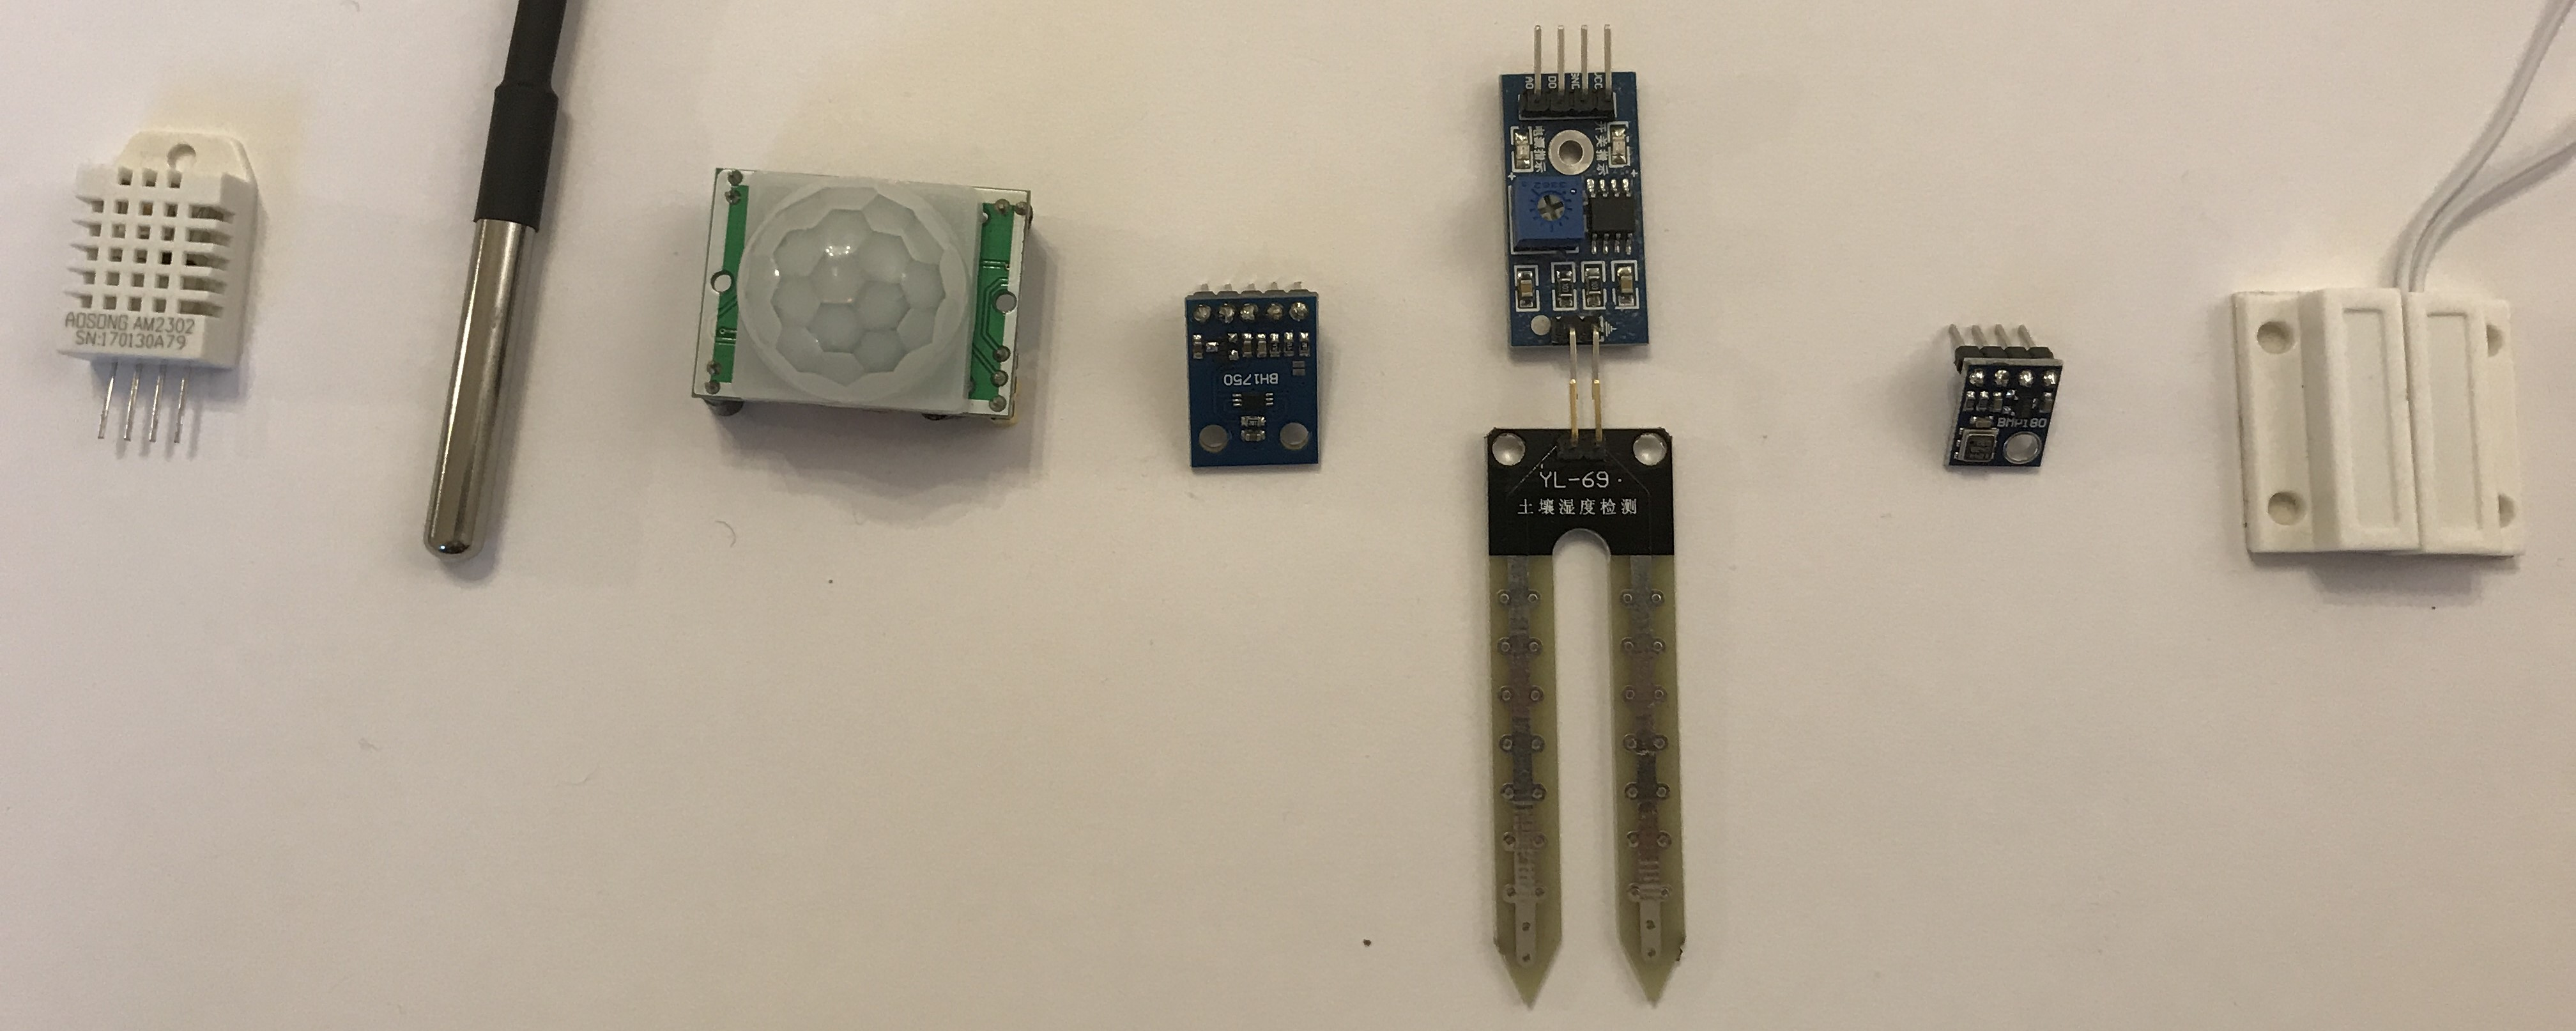
\includegraphics[width=1\textwidth]{bilder/sensoren}
	\caption[Verwendete Sensoren]{Verwendete Sensoren(beginnend von Links): DHT22, DS18B20, PIR-Sensor, BH1750, Bodenfeuchtigkeitssensor, BMP180  und Reed-Kontakt}
	\label{img:verwendeteSensoren}
\end{figure}

\paragraph{DHT11 / DHT22} Bei diesem Sensor handelt es sich um zwei Sensoren, die zur Erfassung von Lufttemperatur und Bestimmung der Luftfeuchtigkeit genutzt werden können. Die beiden Sensoren unterschieden sich nur in der Messgenauigkeit, wobei der DHT22 der genauere der Beiden ist. Die Luftfeuchtigkeit kann bis auf +/- 2\% und die Temperatur auf +/- 0,5 Grad bestimmt werden. Der Wert wird digital zurückgeliefert. Für die Auswertung (siehe Listing \ref{lst:dht22}) der Sensoren wird eine Bibliothek von Adafruit eingesetzt \cite{adafruit2016dht}.

\lstinputlisting[language=C, firstline=348, lastline=350 ,caption={DHT22 Sensorauswertung },label=lst:dht22]{listings/arduinoSensorSenderMesh.ino}

\paragraph{BMP180} Beim BMP180 handelt es sich um einen Luftdrucksensor der über die $I^2C$ Schnittstelle mit dem Arduino verbunden wird. Der Luftdruck kann zwischen 300 und 1100 hPa bestimmt werden \cite{sensortec2013data}. Zusätzlich lässt sich mit diesem Sensor die Temperatur bestimmen, diese Funktion wird allerdings nicht genutzt. Der Sensorknoten bestimmt nur den Luftdruck mit einer Bibliothek von Adafruit (Listing \ref{lst:bmp180}). 
\lstinputlisting[language=C, firstline=364, lastline=368 ,caption={BMP180 Sensorauswertung },label=lst:bmp180]{listings/arduinoSensorSenderMesh.ino}

\paragraph{BH1750} Dieser Sensor wird für die Messung der Beleuchtungsstärke eingesetzt, diese wird in Lux gemessen. Der Sensor unterstützt eine Messung im Bereich zwischen 1 und 65535 Lux, bei einer Auflösung von einem Lux. Der Sensor kann wie der BMP180 über die $I^2C$ Schnittstelle angeschlossen werden. Die Adresse auf der der Sensor erreichbar ist, ist einstellbar. Die Adresse lautet entweder \textit{0x23h} (0 Volt an ADDR- Pin) oder \textit{0x5Ch} (3,3 Volt an ADDR-Pin). 
\paragraph{PIR Sensor} Zur Erkennung von Bewegung wird ein Bewegungsmelder eingesetzt. Der PIR Sensor hat einige Einstellungsmöglichkeiten. Es besteht die Möglichkeit, die Sensitivität und die Dauer des Signals einzustellen. Der PIR Sensor benötigt im Gegensatz zu den vorherigen Sensoren eine Betriebsspannung von 5V. Der Messwert wird einfach mit einem digitalen Eingang gemessen. Eine Nachricht an den Raspberry Pi (Messwertintervall 1min) wird erst nach dem erstmaligen Auslösen des Bewegungsmelders gesendet.
\paragraph{Bodenfeuchtigkeitssensor} Der Bodenfeuchtigkeitssensor verfügt über zwei Ausgänge. Ein Ausgang ist digital und kann mit einem Drehregler direkt am Sensor eingestellt werden. Der Sensor löst beim digitalen Betrieb ab dem definierten Schwellwert aus. Zusätzlich zum digitalen Ausgang liefert der Sensor noch einen analogen Wert, dieser wird dann in einen prozentualen Wert gewandelt (siehe Listing \ref{lst:soilMoisture}). 
\lstinputlisting[language=C, firstline=369, lastline=372 ,caption={Bodenfeuchtigkeit Sensorauswertung },label=lst:soilMoisture]{listings/arduinoSensorSenderMesh.ino}

\paragraph{Reed-Kontakt} Für die Erkennung ob ein Fenster/Tür geschlossen oder geöffnet ist, wurde ein Reed-Kontakt eingesetzt. Dieser fungiert als eine Art Schalter, der ausgelöst wird sobald ein Magnet außerhalb der Reichweite des Reed-Kontaktes ist. Auf dem Sensorknoten sind zwei unterschiedliche Reed-Kontakte installiert. Bei einem kann nur zyklisch überprüft werden ob der Kontakt geschlossen oder geöffnet ist. Der zweite ist an einem Pin mit Interrupt Funktion angeschlossen. Wird dieser ausgelöst wird der Interrupt Service Routine abgearbeitet. Die Nachricht ob ein Reed-Kontakt ausgelöst wurde wird allerdings nur zyklisch abgeschickt. Hierfür wird in jedem Zyklus der Alarm zurückgesetzt und der Interrupt wieder aktiviert, sobald der Reed-Kontakt ausgelöst wurde (siehe Listing \ref{lst:ReedKontakt}). Ein Interrupt wird immer bei wechseln des Signals ausgelöst, das heißt entweder bei einer fallenden oder steigenden Flanke des Signals.
\lstinputlisting[language=C, firstline=383, lastline=389 ,caption={Reed-Kontakt Sensorauswertung },label=lst:ReedKontakt]{listings/arduinoSensorSenderMesh.ino}
\paragraph{DS18B20} Beim DS18B20 handelt es sich um einen Temperatur Sensor, der sowohl die Lufttemperatur messen kann als auch die Bodentemperatur bestimmen kann. Der gesamte Sensor ist in einem wasserdichten Gehäuse. Der Sensor kann über die 1-Wire Schnittstelle angesprochen werden. Dadurch können mehrere Sensoren hintereinander gehängt werden. Diese benötigen eine Datenleitung sowie ein GND und 3,3 V bzw. 5V Leitung. Es können Temperaturen zwischen -55 Grad bis zu 125 Grad mit einer Messgenauigkeit von +/- 0,5 Grad gemessen werden. Jeder Sensor besitzt eine eindeutige und einmalige 64-Bit Seriennummer. An den Sensorknoten können beliebig viele 1-Wire Temperatursensoren angeschlossen werden. Es wird nachdem alle Messwerte von den 1-Wire Sensoren bestimmt wurde jeder Messwert einzeln verschickt (siehe Listing \ref{lst:oneWire}).
\lstinputlisting[language=C, firstline=329, lastline=332 ,caption={1-Wire Sensorauswertung },label=lst:oneWire]{listings/arduinoSensorSenderMesh.ino}
